\documentclass[10pt]{article}
\usepackage{amsmath}
\usepackage[hidelinks]{hyperref}
\usepackage{amssymb}
\usepackage{tikz}
\usepackage{caption}
\usepackage{graphicx}
\graphicspath{{.}}
\usepackage{listings}
\usepackage{verbatim}
\lstset{
language=[LaTeX]TeX,
backgroundcolor=\color{gray!25},
basicstyle=\ttfamily,
columns=flexible,
breaklines=true
}
\captionsetup{labelsep=space,justification=justified,singlelinecheck=off}
\reversemarginpar
\usepackage[paper=a4paper,
            %includefoot, % Uncomment to put page number above margin
            marginparwidth=20mm,      % Length of section titles
            marginparsep=0.8mm,       % Space between titles and text
            margin=12mm,              % 25mm margins
            includemp]{geometry}

\begin{document}
\section*{}
\begin{flushleft}
CSCI 5502 - Data Mining - Homework 1\\
Name: Krishna Chaitanya Sripada\\
Student ID: 104375417\\
Honor Pledge: On my honor, as a University of Colorado at Boulder student, I have neither given nor received unauthorized assistance on this work.
\end{flushleft}
\section*{Ans 1.}
\begin{flushleft}
\textbf{Dataset- I}\\
\vspace{1em}
1. URL: \url{http://networkrepository.com/aff_amazon_copurchases.php}\\
\vspace{1em}
2. This is the Amazon's co-purchase network where the data is about Amazon's ``People who bought X also bought Y" product. Nodes in the dataset represent products purchased and an edge from one node to the other represents that product X is frequently co-purchased with product Y. The data object here is the product items (data points) i.e., the total number of unique products purchased which is 403.4K. The attribute here is the product\_ID. The attribute type here is ratio-scaled numeric attributes which represents the number of times a particular product has been co-purchased, which two product(s) have been frequently co-purchased. \\
\vspace{1em}
3. Based on the frequency of co-purchases of the products, we could find out the number of customers who co-purchased two particular products. The associations between the products could be found out for e.g: the chance of product X and product Y being co-purchased. Also transitivity patterns such as if product X and product Y were co-purchased and product Y and product Z were co-purchased, then product X and product Z might be closely related as well. Interclass cluster similarity could be looked into to find out which product has more co-purchased count when compared to the other products in a cluster.\\
\vspace{1em}
4. This knowledge can be used as a recommendation system that helps improve business intelligence.\\
\vspace{1em}
\textbf{Dataset- II}\\
\vspace{1em}
1. URL: \url{http://networkrepository.com/web_google_dir.php}\\
\vspace{1em}
2. This is Google's web directory which contains details regarding the web-pages and the hyperlinks between pages. Nodes in the dataset represent web-pages in the internet and an edge from one web-page to another represents the relationship between the content in both the web-pages. The data objects here are the web-pages (data points) i.e., the total number of webpages available as per this dataset is 875.7K. The attribute here is the web page ID. The attribute type here is ratio-scaled numeric attributes which represent the number of hyperlinks from one webpage to the other.\\ 
\vspace{1em}
3. Based on the number of links present in one webpage to the other, we could find out the relationship between the pages that have links. The associations analysis such as support and confidence can be found out between different related web-pages. There could be links between pages which have similar content context thus Intraclass cluster similarity could be looked into to find out how similar the content in the both the linked web pages is.\\
\vspace{1em}
4. This knowledge can be used to design search engines where we can provide a URL as an input to the search engine and it returns the list of related web-pages.\\
\vspace{1em}
\end{flushleft}
\section*{Ans 2.}
\begin{flushleft}
1. \textit{Conference Venue:} KDD `13 \\
\hskip 1em \textit{Paper Title:} FIU-Miner: a fast, integrated, and user-friendly system for data mining in distributed environment.\\
\hskip 1em \textit{Authors and Affiliations:} Chunqiu Zeng, Yexi Jiang, Li Zheng, Jingxuan Li, Lei Li, Hongtai Li, Chao Shen, Wubai Zhou, Tao Li (Florida International University, Miami, Florida, USA) and Bing Duan, Ming Lei, Pengnian Wang (ChangHong COC Display Devices Co.,Ltd, Mianyang, China).\\
\vspace{1em}
2. The authors have implemented a Fast, Integrated and User-friendly system to ease data analysis which is called ``FIU-Miner''.  FIU-Miner allowed users to rapidly configure a complex data analysis task without writing a single line of code. It also helps users conveniently import and integrate different analysis problems. The problem was important and challenging because performing data analysis in a specific domain is not trivial; it often requires complex task configuration, onerous integration of algorithms and efficient execution in distributed environment. So, there was a need to simplify the configuration task and the authors could successfully create a tool to help facilitate the same.\\
\vspace{1em}
3. FIU-Miner is an integrated system that facilitates users to conduct the ad-hoc data mining tasks. The solution was to make the FIU-Miner internally leverages a ``Job Scheduler'' to effectively schedule the data mining jobs and leverage a ``Resource Manager'' to manage the underlying resource management. \\
\vspace{1em}
4. FIU-Miner was deployed as the manufacturing process analysis platform at ChangHong Corporation. This was used to optimize the Plasma Display Panel (PDP) manufacturing process. One common task in the PDP process optimization is to extract important feature combinations that are highly related to the yield ratio. The following were the steps followed: \\
\begin{itemize}
\item PDP dataset was loaded from HDFS by HDFS Data Loader and Data Publisher dispatched the dataset to three different Feature Selection algorithms.
\item Important features were first extracted by the Feature Selection algorithms and then combined by the Stable Feature Selection component to output the stable features.
\item Based on the selected stable features, the Finding Frequent Feature Combinations component was running relatively until the number of frequent feature combinations reached the predefined threshold K.
\item The discovered top-K frequent feature combinations were stored in the database and processed.
\end{itemize}
\end{flushleft}
\section*{Ans 3.}
\begin{flushleft}
a. The code is submitted.\\
\vspace{1em}
b. The scatter plot for the last two attributes is shown below:\\
\begin{figure}[!htb]
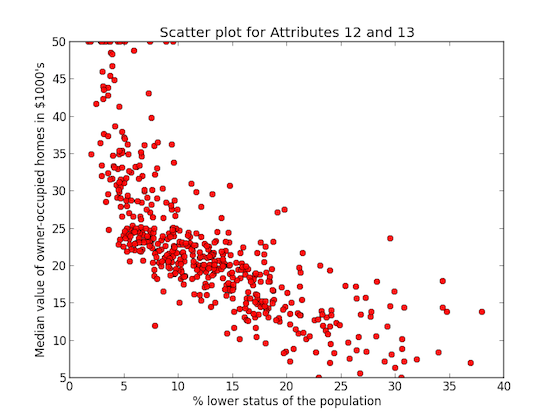
\includegraphics{scatter}
\caption{:Scatter plot for attributes lstat and medv}   
\label{fig::Scatter plot for attributes lstat and medv} 
\end{figure}
\end{flushleft}
\end{document}